% Working draft. Required results and team learning statements remain incomplete.
% Build with an existing TeX environment; do not download packages automatically.
\documentclass[11pt,a4paper]{article}
\usepackage[margin=20mm]{geometry}
\usepackage[T1]{fontenc}
\usepackage{lmodern,microtype}
\usepackage{booktabs,tabularx,array}
\usepackage{enumitem,titlesec}
\usepackage{tikz}
\usetikzlibrary{arrows.meta,positioning}
\usepackage{graphicx,xurl}
\usepackage[hidelinks]{hyperref}
\newcolumntype{Y}{>{\raggedright\arraybackslash}X}
\newcommand{\SourceRevision}{5c33055}
\newcommand{\DraftNote}[1]{\par\smallskip\noindent\textbf{Draft evidence gap:} #1\par}
\setlength{\parindent}{0pt}
\setlength{\parskip}{5pt}
\setlength{\emergencystretch}{1em}
\setlist{nosep,leftmargin=*}
\titlespacing*{\section}{0pt}{9pt}{5pt}
\titlespacing*{\subsection}{0pt}{7pt}{3pt}
\renewcommand{\arraystretch}{1.13}
\makeatletter
\renewcommand{\@oddfoot}{\hfil\small Working draft: 1 November 2026\quad\textbar\quad\thepage\hfil}
\makeatother
\hypersetup{pdftitle={OpsReplay: CS5224 Final Report Working Draft},pdfauthor={CS5224 Group 26}}

\begin{document}
\begin{minipage}[t]{0.60\linewidth}
{\LARGE\bfseries OpsReplay}\\[3pt]
Learn production failures by investigating them.
\end{minipage}\hfill
\begin{minipage}[t]{0.38\linewidth}
\raggedleft\small\textbf{CS5224 Final Report Draft}\\Group 26
\end{minipage}
\par\smallskip
{\footnotesize Lee Hao Zhe, Neeraj Kumbar, Neo Qi Hao, Poh Yu Wen, See Yang Zhi, Teo Kai Xiang\par}
\smallskip\hrule\smallskip
\textbf{Theme: cloud-based production-engineering education.}
OpsReplay provides browser-based individual practice using real, deliberately
misconfigured services. A learner investigates an alert, repairs the fault,
observes measured recovery, then reviews a deterministic debrief and synchronized
recording. This draft describes merged source \texttt{\SourceRevision}; test
revisions and limits are stated separately. Required evaluations remain incomplete.

\section{Motivation and Business Case}
Students and junior software, DevOps and SRE engineers rarely have safe access to
production incidents for practice. A postmortem explains a failure after the event.
It does not require the reader to select evidence under uncertainty or test a
recovery decision. OpsReplay makes these decisions observable in a repeatable
exercise. The intended benefit is better diagnosis and recovery judgement;
learning effectiveness must be measured.

Google's Wheel of Misfortune uses previous incidents for response drills
\cite{sre}. Interactive incident training already exists. OpsReplay's positioning
is a combined investigation, measured consequence, debrief and playback workflow,
with Learn and Code Review as related practice. This is a value hypothesis, not a
claim that the category is new.

\begin{tabularx}{\linewidth}{@{}p{30mm}Y@{}}
\toprule
\textbf{Reference} & \textbf{Relevant distinction}\\
\midrule
Google SRE & Facilitated drills derived from previous incidents.\\
SadServers & Real Linux/DevOps troubleshooting environments and validation \cite{sadservers}.\\
SimIncident & Incident-management simulation and response/coordination practice \cite{simincident}.\\
OpsReplay & Individual real-service investigation, external recovery checks,
recorded evidence, playback and deterministic educational feedback.\\
\bottomrule
\end{tabularx}

\subsection{Revenue model and current offer}
Free gives a complete introductory sample, including Challenge debrief, playback
and fresh retries. Pro is proposed at S\$12/month for additional published content
and longer sessions. Institutional seats are a future sales model. The prototype
implements server-owned entitlements and a fixed-window demo grant; it collects
no payment and creates no recurring subscription.

The retained catalogue contains one Free and one Pro Challenge, one Free and one
Pro lesson, and one Free Code Review. The Pro review remains unpublished. This
small library does not establish commercial content value. Pricing, conversion
and willingness to pay remain unvalidated. Section~\ref{sec:cost} explains the
contribution model and heavy-use risk.

\newpage
\section{Architecture and Cloud Delivery}
The implemented product uses real services per attempt. The application state
machine controls admission, readiness, outcome and cleanup; it does not generate
fake metrics or command results. Authored configuration and validators define an
exercise. System behaviour determines the consequences of each command.

\begin{figure}[ht]
\centering
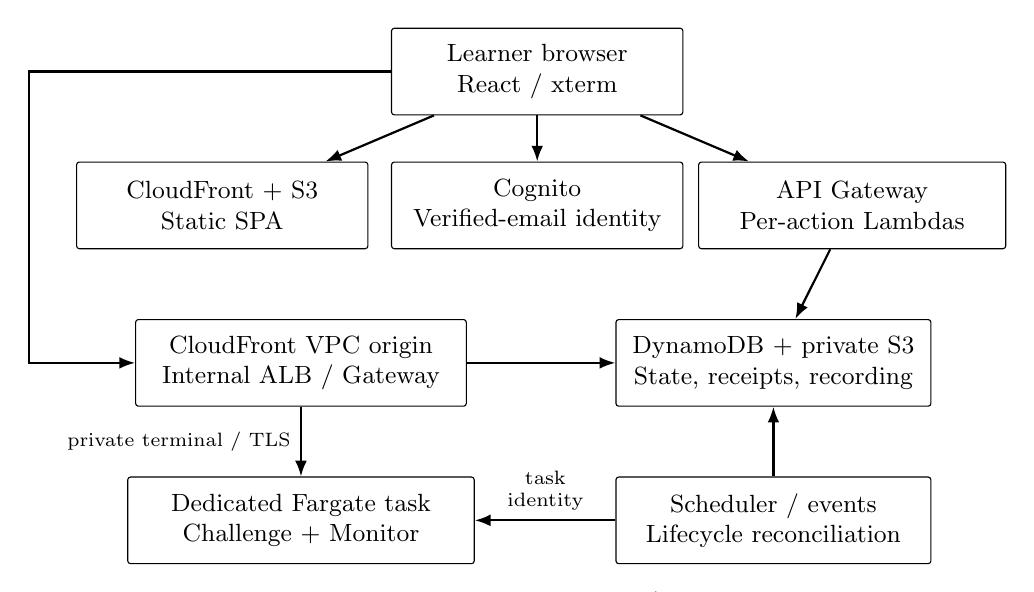
\begin{tikzpicture}[
 box/.style={draw,rounded corners=1pt,align=center,font=\small,minimum height=11mm},
 arrow/.style={-{Latex[length=2mm]},thick}]
\node[box,minimum width=37mm] (browser) at (0,0) {Learner browser\\React / xterm};
\node[box,minimum width=37mm] (static) at (-4,-1.7) {CloudFront + S3\\Static SPA};
\node[box,minimum width=37mm] (auth) at (0,-1.7) {Cognito\\Verified-email identity};
\node[box,minimum width=39mm] (api) at (4,-1.7) {API Gateway\\Per-action Lambdas};
\node[box,minimum width=42mm] (gateway) at (-3,-3.7) {CloudFront VPC origin\\Internal ALB / Gateway};
\node[box,minimum width=40mm] (data) at (3,-3.7) {DynamoDB + private S3\\State, receipts, recording};
\node[box,minimum width=44mm] (task) at (-3,-5.7) {Dedicated Fargate task\\Challenge + Monitor};
\node[box,minimum width=40mm] (lifecycle) at (3,-5.7) {Scheduler / events\\Lifecycle reconciliation};
\draw[arrow] (browser) -- (static);
\draw[arrow] (browser) -- (auth);
\draw[arrow] (browser) -- (api);
\draw[arrow] (browser.west) -- ++(-4.6,0) |- (gateway.west);
\draw[arrow] (api) -- (data);
\draw[arrow] (gateway) -- node[left,font=\scriptsize] {private terminal / TLS} (task);
\draw[arrow] (gateway) -- (data);
\draw[arrow] (lifecycle) -- (data);
\draw[arrow] (lifecycle) -- node[above,font=\scriptsize,align=center,text width=14mm] {task\\identity} (task);
\end{tikzpicture}
\caption{Main delivery paths. Lambda modules are shared in process; functions do
not invoke other Lambda functions. Optional provider calls leave AWS through the
separate assistant action.}
\end{figure}

The static SPA is served from private S3 through CloudFront. Cognito handles
identity and email confirmation. A Regional API Gateway REST API authenticates
owned operations. Each action has its own Lambda bundle, role, timeout and
concurrency setting. DynamoDB transactions protect state and request receipts;
private S3 stores bootstrap material, recordings and content assets.

Terminal WebSockets use CloudFront, a VPC origin, an internal ALB and private
Fargate Gateway tasks. The Gateway reaches the attempt's terminal and independent
Monitor and persists their observations. Challenge tasks have no task IAM role
and no internet route. Private endpoints support required platform-service access.
Secrets and bootstrap permissions are separate from learner-container access.

AWS fits independent, intermittent sessions and class bursts. Fargate adds
isolated compute per attempt; Lambda handles bounded requests. Managed identity,
storage and monitoring reduce operational work. ALB, Gateway and endpoint idle
costs remain material. These benefits do not prove that cloud is cheaper than an
equivalent on-premise service.

\newpage
\section{State, Reliability and Educational Feedback}
\subsection{Admission and lifecycle}
The start action validates identity, input, published content and entitlement.
It first resolves an existing request receipt. A transaction saves the receipt,
active-attempt lock, session, lifecycle entry and immutable launch arguments before
external effects. Content and plan conditions reject stale admission snapshots.
Retries reuse the saved request and ECS launch identity rather than create a
second task. Reconciliation repairs interrupted provisioning and schedules.

\begin{center}
\small
Admitted $\rightarrow$ provisioning $\rightarrow$ ready $\rightarrow$
fixed outcome / drain $\rightarrow$ confirmed cleanup $\rightarrow$ saved result
\end{center}

Readiness requires durable terminal and Monitor observations. The saved grant
fixes the attempt's time limit. The first valid outcome fixes one cutoff; later
end requests return it. Recording coverage permits task cleanup while immutable
page sealing continues. Without coverage, the bounded drain ends in explicit
incomplete recording rather than an invented success. Confirmed task stop and
schedule cleanup precede once-only finalisation and lock release.

Lifecycle events are discovery hints. Workers reread current state before effects.
Conditional writes fence stale generations, late timers and overlapping workers.
Bounded sweeps retain cursors across invocations. Component tests and the
1 November hosted response-loss, reconnect, token-expiry and Gateway-replacement
checks support this design. Larger recovery capacity remains unmeasured.

\subsection{Recording and debrief}
The learner has a root shell in the Challenge container. The separate Monitor
checks actual service recovery; terminal output is never the recovery authority.
The Gateway records terminal bytes, timestamped measurements and file captures
outside the learner's writable environment. Saved page references and sealed
cutoffs support playback and stable results.

Debrief derivation uses pinned authored metadata and recorded evidence. It shows
the root cause, causal chain, observed and missed evidence, possible harmful
actions, outages and recommended recovery. A file-path mention is not evidence
that the file was read. A command preceding an outage does not prove causation.
Captures describe intervals, including possible background changes.

The implementation reports raw components: recovery time, measured request
counters, command count, observed outages and outage duration. It does not invent
a weighted 0--100 score. Incomplete recordings have a null score. Hints and
proposal acknowledgements remain visible assistance information. Learner-writable
shell acknowledgements do not prove execution and do not set numeric scores.
A retry runs a fresh task and preserves the first result.

\subsection{Authority and privacy}
Every owned read and mutation checks identity and access. Public DTOs use explicit
projections. Private manifests, validators, unreleased hints, bootstrap secrets and
unreleased review findings stay out of browser payloads and assistant context. The repository
is public, so these runtime boundaries cannot provide exam secrecy against source
inspection. Image findings and broader availability limits remain open.

\newpage
\section{Web Experience, Content and Assistant}
The main learner path is catalogue, briefing, sign-in, start, investigation,
recovery, debrief, playback and retry. A current-attempt notice explains that
navigation does not pause the incident. Progress states distinguish provisioning,
readiness and result preparation. The briefing documents available services and
known evidence paths without revealing the planted fault.

\subsection{Frontend and Code Review}
The approved neobrutalist discovery design uses IBM Plex typography, dark outlines,
hard shadows and yellow, blue and pink accents. It applies to Home, catalogue and
shared navigation. Mantine controls retain keyboard behaviour. Catalogue filters
and pagination use server metadata; text search is explicitly limited to the
loaded page. Failed reads and empty results have different messages.

Code Review presents source context with selectable lines and inline concerns.
Version-bound learner drafts survive refresh. Deterministic submission matches
flagged lines against authored reference ranges and produces found/missed feedback.
Written concerns appear beside the reference but are not graded. Saved result
URLs and History support later review. Same-request recovery prevents a lost
submission response from producing a second result.

Learn provides original summaries, lessons and links to official incident reports.
Free lessons are static assets. Pro reads require server entitlement. Authored
assets and immutable publication metadata are separate from account grants.

\subsection{Optional assistant}
The Challenge assistant uses the production provider adapter to explain recent
public evidence and optionally return a typed command proposal. Context is bounded
to public service information, completed commands/output, visible metrics, released
hints and recent turns. It never owns truth, recovery, scoring or state transitions.

A proposal requires separate learner confirmation of the exact text. The Gateway
validates ownership, expiry and current input generation. Shell integration checks
that the actual input buffer is empty. Uncertain dispatch is not automatically
resent; manual investigation remains available. A command filter is not a shell
sandbox, and proposal acceptance does not prove successful execution.

Each assistant request reserves one conversation slot and request receipt.
Provider failure and late completion cannot overwrite a newer turn. Streaming
text is provisional until the saved owned turn confirms completion. The browser
states that selected evidence leaves AWS for the configured provider. Credentials
and provider text stay out of logs.

The account owner has confirmed permission for the selected Ark demo account.
The campaign used bounded paid calls under this permission; console cap verification
was not a prerequisite. No enforced billing cap is claimed. Adapter-only timing
and full deployed streams are reported separately below. Gameplay works with the
assistant disabled.

\newpage
\section{System Evaluation}
\label{sec:system}
Evidence is bound to a revision, workload and environment. The 1 November campaign
used \texttt{5c33055}, two new operator-created learners, six attempts, at most two
concurrent Challenge tasks and one Gateway in Singapore, with the US East terminal
edge \cite{release-checkpoint}. The 29 October sign-up and 450-GET results retain
their original \texttt{e59067b} scope \cite{aws-checkpoint}.

\begin{tabularx}{\linewidth}{@{}p{34mm}Y@{}}
\toprule
\textbf{Area} & \textbf{Observed result and scope}\\
\midrule
Identity/access & Hosted PKCE login and fixed-window Pro access passed. Inbox
sign-up, guest denial and ownership checks are 29 October evidence.\\
Request recovery & Lost start response and same-request replay recovered one
attempt. Duplicate active-end requests retained one terminal outcome.\\
Real Challenges & Both recovered for 60 seconds. DNS-only repair left checkout
at 502; a validated reload restored it.\\
Terminal/recovery & Original idle socket survived 610 seconds. Expired token
returned 401; fresh login and reconnect resumed the same attempt.\\
Gateway loss & Replacement recovered the same attempt and recording. The other
disconnected attempt abandoned normally; its deadline check was repeated.\\
Finalization & Deadline, final exports, deletion and cleanup verification are
in progress; the checkpoint records their final status.\\
\bottomrule
\end{tabularx}

\subsection{Bounded API measurements}
One worker sent 150 GETs; two distinct learners sent 300. All 450 passed HTTP,
schema and owned-session identity checks. The mix read catalogue, account and
saved sessions with two-second think time. It did not refresh presence, start
tasks, issue terminal tickets or mutate sessions.

\begin{center}\small
\begin{tabular}{@{}lrr@{}}
\toprule
Endpoint & One worker p50 / p95 (ms) & Two workers p50 / p95 (ms)\\
\midrule
Catalogue & 75 / 249 & 60 / 231\\
Account & 66 / 221 & 54 / 219\\
Session & 71 / 190 & 48 / 208\\
\bottomrule
\end{tabular}
\end{center}
The measured mixes achieved 1.33 and 2.68 requests/second. They do not establish
maximum throughput, provisioning capacity, terminal latency or a classroom limit.

\subsection{Repeatability and later checks}
Historical local reports at \texttt{f89e258} recorded twenty passing Challenge
suite runs and twenty passing Monitor suite runs per incident: eighty suite
executions across the two incidents. Image IDs stayed unchanged. Suite durations
are not learner recovery times, and local Docker is not Fargate.

The later frontend record \cite{frontend-record} reports 26 fixture interaction
checks and no page overflow at eight widths from 320 to 1440 CSS pixels. This is
local UI evidence, not native-mobile or new hosted acceptance. PR \#129 at
\texttt{60f4f7f} passed nine repository jobs and its metadata check, including
ordinary editor/package and Challenge checks. Later package PRs culminated in
merged PR \#135 at \texttt{5c33055}; fresh publications and all six exact-digest
scans passed the scoped campaign gate. Residual findings are listed below.

\newpage
\section{End-user Evaluation and Outstanding Validation}
\subsection{Formative learner protocol}
The prepared pilot targets five to ten computer science students or junior
engineers \cite{pilot}. Each participant uses the complete interactive workflow
for one incident and studies a static explanation for the other. Four assignment
sequences counterbalance condition and order. The assistant is off in both core
conditions. Common tutorial and study times are fixed.

Each condition has baseline questions, twelve minutes of study and post-condition
questions. Interactive study allocates eight minutes to investigation/repair and
four to debrief/playback, pausing separately for result preparation. An unresolved
attempt is ended through the normal UI. Transfer questions test a new case.
Brief product tasks cover Learn, Code Review and saved results; SUS and interviews
assess usability. Total planned participation is approximately 65 minutes.

Report recruited/completed counts, exclusions, experience, assignment, incident,
hints, completion, rubric scores and SUS. Keep interrupted learning scores missing.
Use participant pseudonyms and aggregate examples. Names, consent, identity
mappings and recordings remain in restricted storage outside Git. The facilitator,
contact and deletion date must be set before consent; application deletion and
backup retention must be verified before participant testing.

The upstream incident is Easy and DNS is Medium. Counterbalancing reduces order
effects but does not remove this difficulty difference or carryover. Results must
be separated by incident and condition. A small pilot cannot prove broad learning
effectiveness, retention, or the separate effect of playback.

\DraftNote{No participant results have been supplied for this draft. Agent
acceptance and the owner's informal trial do not replace the planned end-user
evaluation. Add anonymous outcomes and concrete usability changes after the study.}

\subsection{Measured assistant and remaining checks}
Six ordinary synthetic cases were planned for three repeats. The original run
attempted 11 calls with one failure; an explicit eight-call supplement completed
the missing repeats. The pooled baseline has 19 attempts, 18 completions and one
failure (5.26\%). Completed adapter latency was p50 4616 ms / p95 6013 ms.
The failed stream was not captured; a separate successful diagnostic does not
establish its cause. Injection and hidden-answer fixtures were excluded.

Agent manual rubric review found relevant proposals in 18/18 completed replies,
teaching accuracy in 17/18 and unsupported facts in 4/18. No destructive proposal
was found in these ordinary cases. These are separate dimensions, not independent
human grades. PR \#137 clarifies socket ownership and tested versus loaded
configuration. Two targeted calls made the distinction explicit but do not
establish post-fix accuracy; deployed tests retained pre-fix source.

Two deployed streams completed in 8574 and 6643 ms. First text arrived at 5019 ms
in the first call. The second was tool-only; saved fallback text is not a provider
delta or the requested explanation. Both required confirmation; repeating the
second counted once. A helper's wrong \texttt{completed} assertion was reconciled
against the contract's saved \texttt{accepted} receipt.

Reported tokens give US\$0.0073083 baseline and US\$0.0011263 deployed estimates
at dated rates/FX; the failed baseline call retains a separate US\$0.0013201
reservation. Diagnostic/fix calls are separate. No invoice, population p95,
security-benchmark or accuracy guarantee is claimed \cite{release-checkpoint}.

\subsection{Security and availability limits}
Fresh scans of four Gateway/Monitor images reported no findings. Each Challenge
reported one HIGH, three MEDIUM and three LOW; no CRITICAL or UNKNOWN findings.
Three glibc findings map to new owner acceptance for isolated root learners; four
lower findings remain outside it. The expired 29 October exception was not reused.
The checkpoint records digests and conditions. Production clearance, larger
concurrency, native-mobile use and recovery capacity remain unverified.

\newpage
\section{Cost and Equivalent On-premise Hosting}
\label{sec:cost}
Use list prices before credits, discounts and taxes, and separate measured
resource use from projections. The two historical Challenge intervals totalled
1,438 seconds. At the documented Singapore rate for 1 vCPU and 2 GiB,
US\$0.06162/hour, their task-only compute estimate is US\$0.0246. This excludes
Gateway, ALB, endpoints, WAF, requests, logs and storage. It is not an invoice.

One Gateway, three interface endpoints in two availability zones and one internal
ALB project to US\$97.83/month at 730 hours before usage charges
\cite{pricing-record,aws-fargate,aws-vpc,aws-alb}. Idle shared infrastructure can
dominate a small SaaS. An account-wide estimated billing observation cannot be
treated as campaign-attributed final spend.

\subsection{Pricing and contribution assumptions}
The S\$12 proposal uses a planning FX rate of S\$1.35/US\$1, six paid Challenge
hours/month, US\$0.30 assistant and US\$0.15 API/storage allowance per subscriber.
Five active Free users per subscriber each use 0.5 hours plus US\$0.075 other
delivery allowance. The combined variable delivery cost is S\$1.82.

Future domestic card and optional Billing fees are modelled as 4.1\% + S\$0.50
\cite{stripe}. No such fees are incurred by the demo. Under these assumptions,
\[
\mbox{Contribution} = 12 - 1.8208395 - (12\times0.041+0.50)
                    \simeq \mbox{S\$9.19 per paid subscriber}.
\]
The fixed allocation is S\$972.07/month: shared infrastructure S\$132.07,
other shared use S\$40, content/support S\$600 and acquisition S\$200.
Operating break-even is 106 subscribers. Infrastructure-only break-even is 19;
these are different quantities. At 60 paid runtime hours, contribution falls to
S\$4.70 and operating break-even rises to 208. Costs exclude engineering payroll,
startup recovery and tax. These are scenarios, not measured profit.

Finite attempts do not cap monthly compute. The prototype must not promise
unlimited paid runtime. A production offer needs usage evidence and a funded
capacity/heavy-user policy. The small environment guard is an operational limit,
not a justified commercial service guarantee.

\subsection{Fair comparison model}
Compare the same images, attempt workload, recording retention and external
provider cost. An on-premise container host must reserve capacity for Gateway,
Monitor and the measured peak attempts, with equivalent network/identity and
storage controls. Do not treat one laptop demonstration as equivalent service
capacity or compare a single host with multi-zone cloud availability.

\begin{tabularx}{\linewidth}{@{}>{\raggedright\arraybackslash}p{27mm}Y@{}}
\toprule
\textbf{Cloud cost} & Shared Gateway/ALB/endpoints + measured task-hours + API,
Lambda, DynamoDB, identity, storage/transfer and monitoring + operating labour.\\
\textbf{On-premise cost} & Hardware amortisation + measured power + network,
backup/storage, identity and maintenance + operating labour.\\
\textbf{Both} & The same external LLM usage and content/support costs. Include
the capacity and availability level provided by each configuration.\\
\bottomrule
\end{tabularx}

\DraftNote{Final attributed AWS charges, equivalent-host quote/lifetime, measured
host capacity/power, network and staff assumptions are missing. Complete steady
use and class-burst comparisons before drawing a hosting-cost conclusion.}

\newpage
\subsection{On-premise service boundary and sensitivity}
The code uses AWS SDKs for state, object storage, identity, task launch and timers.
Running the three images on a server does not supply the complete SaaS. An
equivalent deployment needs authenticated HTTPS ingress and action workers;
verified-email identity; a transactional store with conditional request receipts
and leases; private immutable recordings and backups; isolated task scheduling;
durable deadline/reconciliation workers; and monitoring, secrets and deployment
controls. DynamoDB Local tests do not establish a production state-store substitute.
These are comparison requirements, not added MVP services.

SP Group lists S\$0.2859/kWh before GST for Q4 2026 \cite{sp-tariff}.
A Singapore T350 retail listing displays S\$4,955.80 for a Xeon E-2324, 8 GB RAM,
2 TB HDD and non-redundant PSU \cite{host-listing}. Its memory/storage upgrades,
tax, delivery and current availability require a qualified quote. Neither this
listing nor maximum server specifications prove that the machine can host the
complete workload. PSU capacity is not average power draw.

Define a working case with two simultaneous attempts, 730 platform hours/month
and total billable Challenge hours $H$. Use S\$4,000 capex over 36 months as a
sensitivity input, not the quoted configuration. Assume 100 W average draw,
1.4 power/cooling overhead, S\$50 network, S\$30 backup and S\$20 maintenance
per month. Assume cloud operations take two hours/month and on-premise six, at
S\$30/hour. Allow 60 hours of initial adapter work over 36 months. All inputs
except the tariff and documented AWS rates are assumptions.

\[
\begin{array}{l}
 C_{\rm cloud}=132.066855+0.083187H+40+60,\\
 C_{\rm premise}=4000/36+0.1(730)(0.2859)(1.4)+50+30+20+180+50.
\end{array}
\]

\begin{center}\small
\begin{tabular}{@{}rrr@{}}
\toprule
Challenge hours/month & Cloud projection (S\$) & On-premise working case (S\$)\\
\midrule
50 & 236.23 & 470.33\\
400 & 265.34 & 470.33\\
1200 & 331.89 & 470.33\\
\bottomrule
\end{tabular}
\end{center}

The table excludes equal external provider and content costs. Assigned labour
and port effort materially affect it. At the same two hours of operations,
on-premise falls to S\$350.33. With that labour and an already qualified deployment
requiring no adapter work, it falls to S\$300.33, below cloud at 1,200 hours.
This is not measured evidence that either host is cheaper.

The base algebraic crossing is about 2,864 hours, beyond two tasks' 1,460-hour
monthly arithmetic ceiling. Do not claim that crossing is achievable. The
equal-labour, no-port case crosses near 821 hours, but peak capacity still needs
measurement. Monthly hours alone cannot size a class burst. A larger host changes
capex and power. A single non-redundant server also has different availability
from managed multi-zone storage; backups do not provide continuous failover.
The supporting working model records S\$1,000/S\$8,000 capex sensitivity and
required qualification evidence. Final comparison must use actual workloads,
power, operator time, availability and attributed cloud charges.

\newpage
\section{Code Explanation, Disclosure and Conclusion}
\subsection{Repository and component boundaries}
Public code: \url{https://github.com/ehz0ah/OpsReplay}. Keep this URL accessible
until marks and feedback are released. This draft uses merged commit
\texttt{\SourceRevision}. The public checkpoint records
bind older measurements to their own commits.

\begingroup\small
\begin{tabularx}{\linewidth}{@{}>{\raggedright\arraybackslash}p{39mm}Y@{}}
\toprule
\textbf{Path} & \textbf{Role and useful entry point}\\
\midrule
\texttt{apps/web/} & React routes, Mantine controls, xterm workspace, account
callback, learner drafts, evidence and playback views.\\
\texttt{apps/api/src/} & One action per handler/bundle: start/end, tickets,
catalogue/account, content, review, history and assistant. Start saves admission
receipts before provisioning.\\
\texttt{packages/session/} & Shared lifecycle, recording coordination and
deterministic debrief derivation. \texttt{src/finalise.ts} binds saved evidence to
the pinned debrief and commits the result once.\\
\texttt{apps/gateway/} & Owned terminal connections, generation checks,
measurements, recording persistence and confirmed proposal delivery.\\
\texttt{apps/monitor/} & Independent probes, sustained recovery, timestamped
metrics and watched-file capture. Learner output cannot declare recovery.\\
\texttt{content/} & Authored Challenge assets and Learn/review material.
Publication validates and pins versions; public reads use restricted projections.\\
\texttt{packages/contracts/} & JSON Schema, OpenAPI, generated public types and
private recording/lifecycle contracts. Examples and checks track wire behaviour.\\
\texttt{infra/} & CDK stacks for durable resources, hosting, session actions,
private environments, events and teardown-safe deployment settings.\\
\texttt{scripts/evaluation/} & Revision-bound scenario repeats, GET/terminal
measurements and assistant evaluation. Live operations require explicit runs.\\
\bottomrule
\end{tabularx}
\endgroup

\subsection{Verification and operation}
Node 22 and existing project dependencies are required. \texttt{npm run quality}
checks lint, formatting and types; \texttt{npm run check} checks contracts and
support tooling. Component tests cover API, Gateway, Monitor, content, web and CDK.
Image and DynamoDB Local integrations are separate requirements. Local results
do not verify AWS IAM, managed transport, billing or provider behaviour.

Deployment pins approved images and enables runtime only for a scoped window.
Admission is stopped before drain; both demo upgrade and Gateway runtime must be
disabled in teardown. Durable learner results are preserved unless their deletion
is explicitly requested and verified. Test artifacts with identities or provider
data remain outside Git.

\subsection{AI-use disclosure}
AI assistance was used to propose implementation code, tests, UI refinements,
review fixes and this report draft. Proposed changes were checked against source,
contracts and test evidence. AI-generated summaries do not constitute measured
results. The team must verify the final disclosure against its own contributions.
\DraftNote{Add the team's own verified statement of what it learned from AI use.
Do not submit an invented personal-learning statement.}

\subsection{Conclusion}
OpsReplay implements a complete browser-based investigation and saved-feedback
workflow, with bounded AWS acceptance evidence. Its strongest completed technical
work is isolated real-service practice, duplicate-safe lifecycle handling and
evidence-based debrief/playback. Exact-image qualification and bounded paid
assistant measurements now have current evidence. The learner study, final
hosting-cost evidence and rehearsal remain required for presentation readiness.

\newpage
\begin{thebibliography}{99}
\small
\bibitem{sre} Google SRE, ``Postmortem Culture: Learning from Failure.''
\url{https://sre.google/workbook/postmortem-culture/}.
\bibitem{sadservers} SadServers, ``FAQ.'' \url{https://sadservers.com/faq}.
\bibitem{simincident} SimIncident. \url{https://simincident.com/}.
\bibitem{aws-checkpoint} OpsReplay, ``SaaS AWS checkpoint, 29 October 2026.''
\url{https://github.com/ehz0ah/OpsReplay/blob/4df4842cf79a8f662b309bb778a9dc5765d29c6a/docs/checkpoints/2026-10-29-saas-aws.md}.
\bibitem{release-checkpoint} OpsReplay, ``Release qualification, 1 November 2026,''
tested source \texttt{5c33055}.
\url{https://github.com/ehz0ah/OpsReplay/blob/main/docs/checkpoints/2026-11-01-release-qualification.md}.
\bibitem{frontend-record} OpsReplay, ``Neobrutalist discovery pages,''
31 October 2026.
\url{https://github.com/ehz0ah/OpsReplay/blob/4df4842cf79a8f662b309bb778a9dc5765d29c6a/docs/decisions/neobrutalist-discovery.md}.
\bibitem{pilot} OpsReplay, ``Formative learner study,'' protocol.
\url{https://github.com/ehz0ah/OpsReplay/blob/4df4842cf79a8f662b309bb778a9dc5765d29c6a/docs/evaluation/pilot/README.md}.
\bibitem{evaluation-tools} OpsReplay, ``Run reproducible evaluations,''
including 31 October benchmark corrections.
\url{https://github.com/ehz0ah/OpsReplay/blob/4df4842cf79a8f662b309bb778a9dc5765d29c6a/docs/runbooks/evaluation-tools.md}.
\bibitem{pricing-record} OpsReplay, ``Pricing proposal,'' 26 October 2026.
Rates and commercial assumptions are the dated proposal inputs.
\url{https://github.com/ehz0ah/OpsReplay/blob/4df4842cf79a8f662b309bb778a9dc5765d29c6a/docs/decisions/pricing-proposal.md}.
\bibitem{aws-fargate} AWS, ``AWS Fargate Pricing.''
\url{https://aws.amazon.com/fargate/pricing/}.
\bibitem{aws-vpc} AWS, ``Amazon VPC Pricing.''
\url{https://aws.amazon.com/vpc/pricing/}.
\bibitem{aws-alb} AWS, ``Elastic Load Balancing Pricing.''
\url{https://aws.amazon.com/elasticloadbalancing/pricing/}.
\bibitem{stripe} Stripe Singapore, ``Pricing.''
\url{https://stripe.com/en-sg/pricing}.
\bibitem{sp-tariff} SP Group, ``Tariff Information,'' Q4 2026, read 31 October 2026.
\url{https://www.spgroup.com.sg/our-services/utilities/tariff-information}.
\bibitem{host-listing} Sim Lim Square / Bizgram, ``Dell PowerEdge T350,''
retail listing read 31 October 2026. Configuration and price require confirmation.
\url{https://www.simlimsquare.com.sg/product/dell-poweredge-t350-poweredge-t350-xeon-e-2324-1x8gb-dim-9850}.
\end{thebibliography}
\end{document}
